\newcommand{\figblocks}{
\begin{figure}
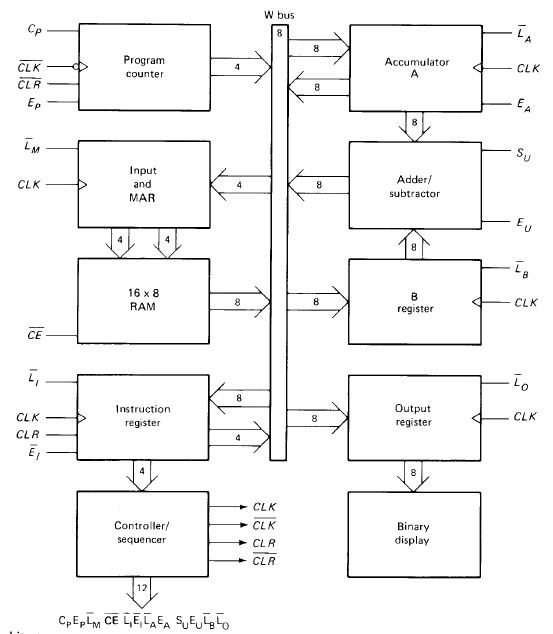
\includegraphics[width=0.6\linewidth]{figures/blocks.jpg}
\caption{Diagrama de blocos do processador SAP1. \cite{malvino}}
\label{f-blocks}
\end{figure}
}

\newcommand{\figblockmux}{
\begin{figure}
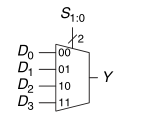
\includegraphics[width=0.5\linewidth]{figures/42-mux.png}
\caption{Bloco representando circuito multiplexador 4:2.}
\label{f-42mux}
\end{figure}
}

\newcommand{\fighmux}{
\begin{figure}
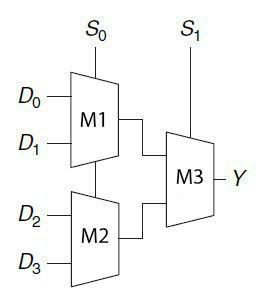
\includegraphics[width=0.5\linewidth]{figures/h-mux.jpg}
\caption{Diagrama de circuito multiplexador 4:2 construido hierarquicamente usando 3 multiplexadores 2:1.}
\label{f-hmux}
\end{figure}
}

\newcommand{\figcd}{
\begin{figure}
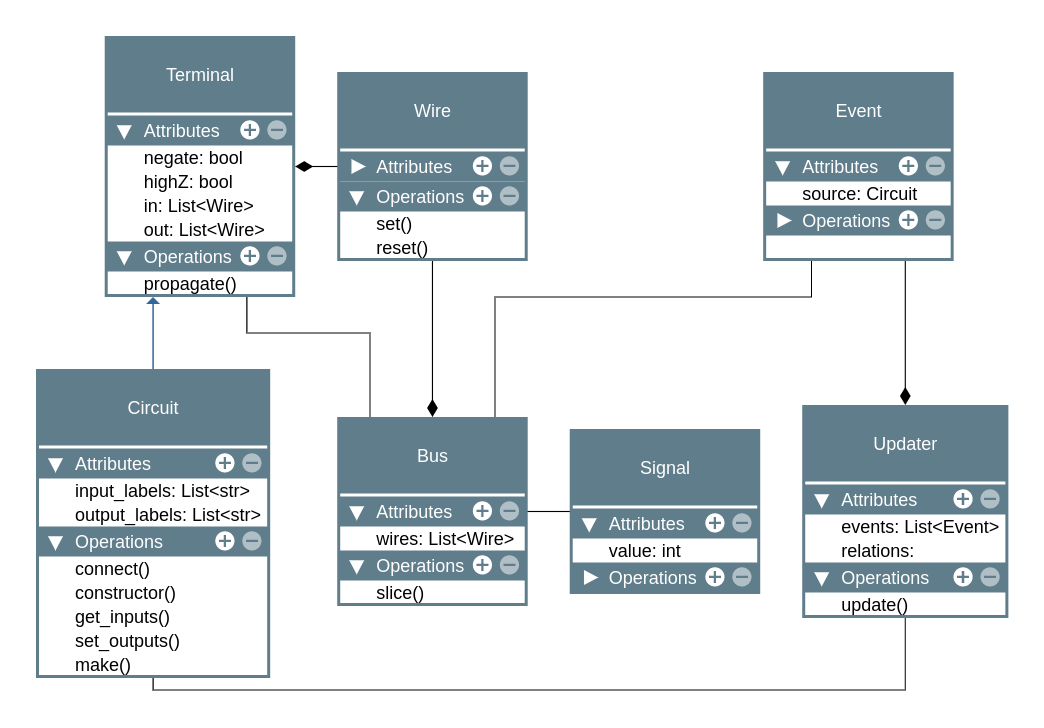
\includegraphics[width=\linewidth]{figures/class-diagrams.png}
\caption{Diagrama de classes para ferramenta.}
\label{f-cd}
\end{figure}
}

\newcommand{\logo}{

\includegraphics[width=0.3\textwidth]{figures/uninter-logo.png}\\
}

\newcommand{\parecer}{
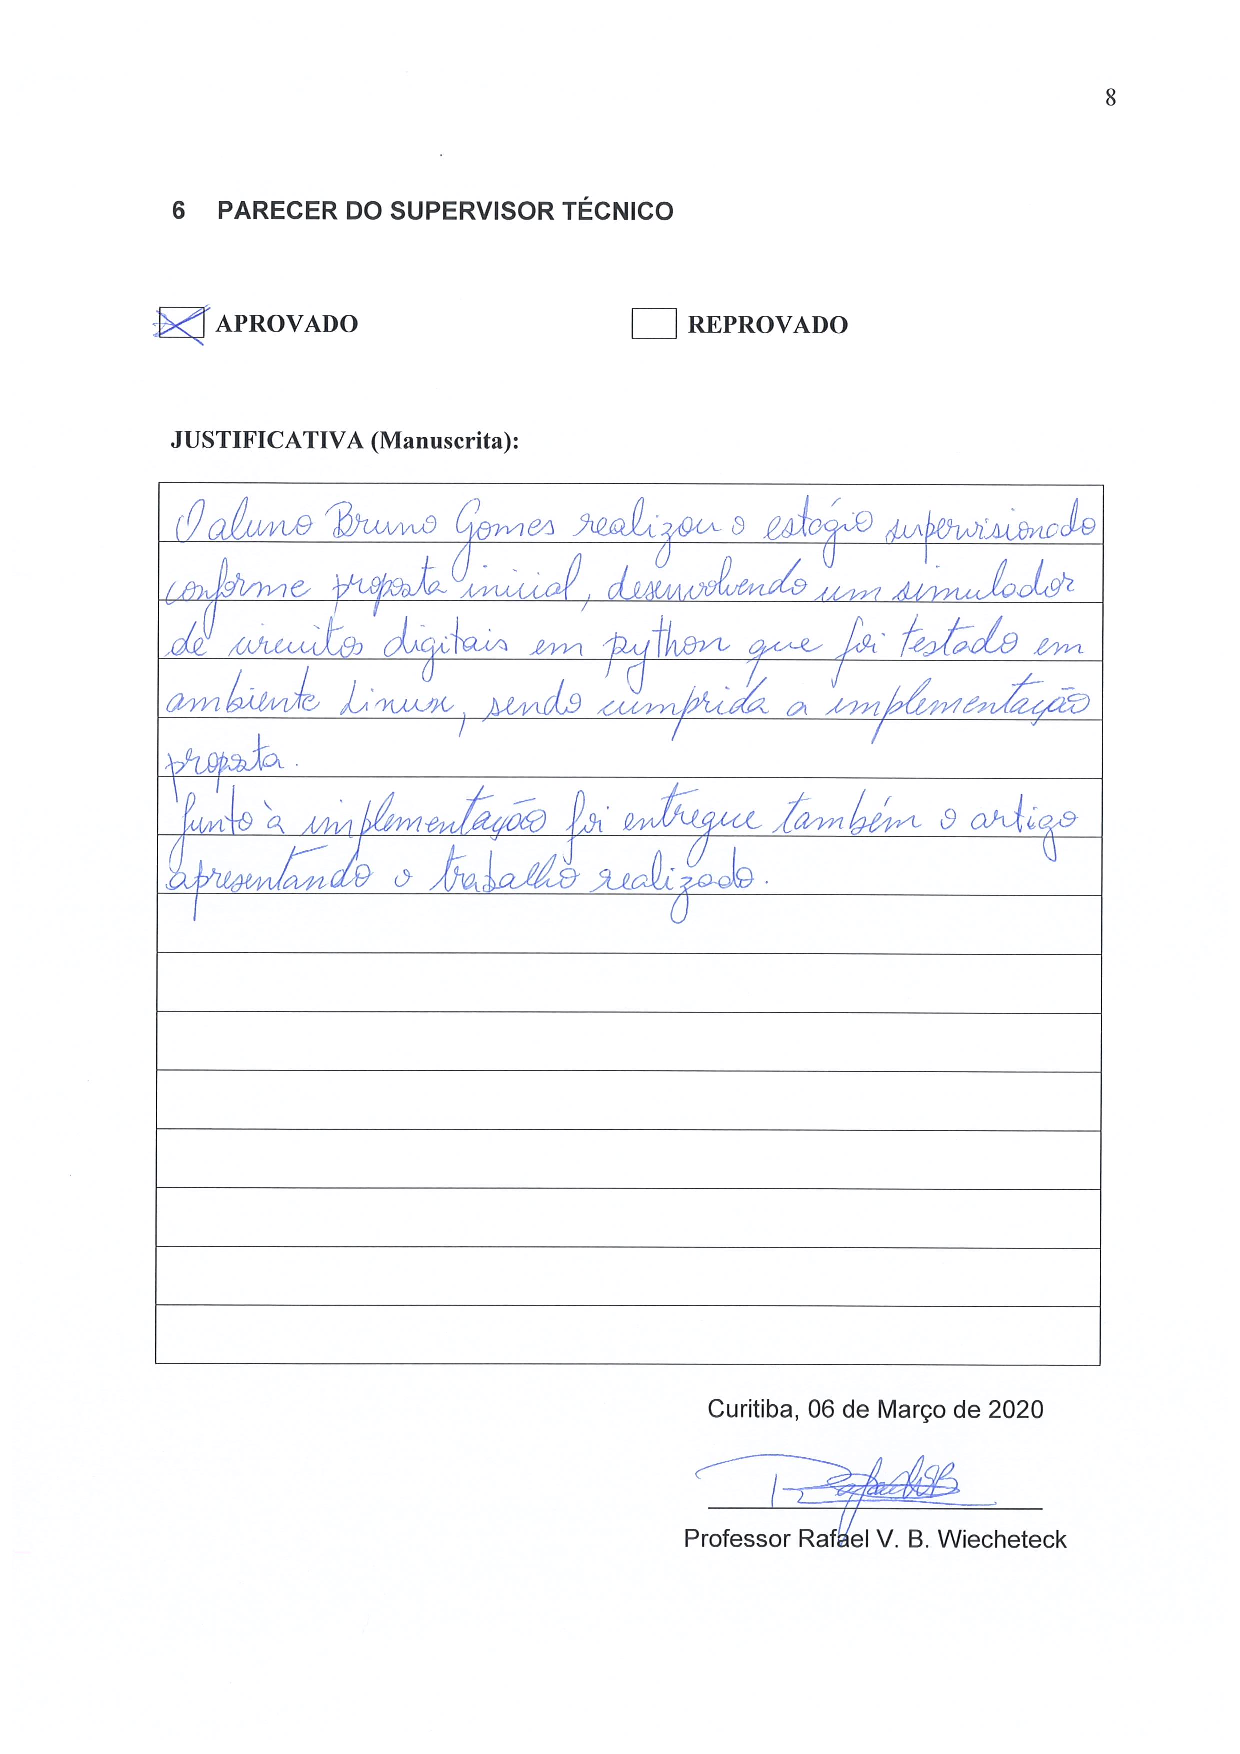
\includepdf[pages=-]{figures/parecer-tecnico.pdf}
}
